\section{Ziel}
\label{sec:Zielsetzung}
In diesem Versuch wird eine Wärmepumpe untersucht. Es sollen die reale Güteziffer dieser und die mechanische Leistung, die erbracht wird, berechnet werden. 
Diese kann man dann mit der Güteziffer einer theoretischen, idealen Wärmepumpe und den Messwerten der Leistung vergleichen und somit die Effizienz der realen Wärmepumpe diskutieren.
\section{Theorie}
\label{sec:Theorie}
Typischer Weise gleichen sich die Temperaturen zweier Reservoire immer an. Meist aber ist es von größerem Interesse sehr kalte oder sehr warme Stoffe zu betrachten, um neue Erkenntnisse
zu erlangen. Daher benötigt man eine Methode dies zu realisieren. Eine Methode ist die Nutzung einer Wärmepumpe. Denn durch eine Wärmepumpe ist es möglich die (Wärme-)Energie aus 
einem niederenergetischen Reservoir in ein höherenergetisches Reservoir zu "pumpen". Betrachtet man beispielsweise zwei Behälter einer Flüssigkeit, ermöglicht es eine Wärmepumpe 
die Temperatur eines der Reservoire zu senken und gleichzeitig die des Anderen zu erhöhen. 
\subsection{Das Prinzip einer Wärmepumpe}
\label{subsec:Prinzip}
Wie bereits erwähnt ermöglicht es eine Wärmepumpe die natürliche Flussrichtung der Wärmeenergie umzukehren. Um dies zu realisieren muss man allerdings zusätzlich Energie in das System
einfließen lassen. Typischer Weise wird dies durch mechanische Arbeit erbracht.


Für eine solche Wärmepumpe wird die Güte
\begin{equation}
    \label{eqn:Güte_ideal}
    \nu_{\text{ideal}} = \frac{Q_1}{A} = \frac{T_1}{T_1 - T_2}
\end{equation}
als Eigenschaft der Wärmepumpe definiert. Hierbei beschreibt $Q_1$ die abgegebene Wärmemenge des "kalten"\: Reservoires und A die mechanische Arbeit die in das System eingebracht wird.
Somit beschreibt die Güte das Verhältnis zwischen transportierter Wärme und aufgebrachter mechanischer Arbeit. 


Aus dem zweiten Hauptsatz der Thermodynamik folgt für eine Wärmepumpe der Zusammenhang $\frac{Q_1}{T_1} - \frac{Q_2}{T_2} = 0$. Daraus kann gefolgert werden, dass die Wärmeübertragung 
immer reversibel verlaufen muss. Dies ist allerdings nur eine theoretische Forderung, welche nicht realisiert werden kann, da es immer gewisse Energieverluste gibt. Daher lässt sich
lediglich die Aussage treffen 
\begin{equation*}
    \label{eqn:Güte_real}
    \nu_{\text{real}} \textless \nu_{\text{ideal}}
\end{equation*}

\subsection{Die Arbeitsweise einer Wärmepumpe}
\label{Arbeitsweise}
\begin{figure}
    \centering
    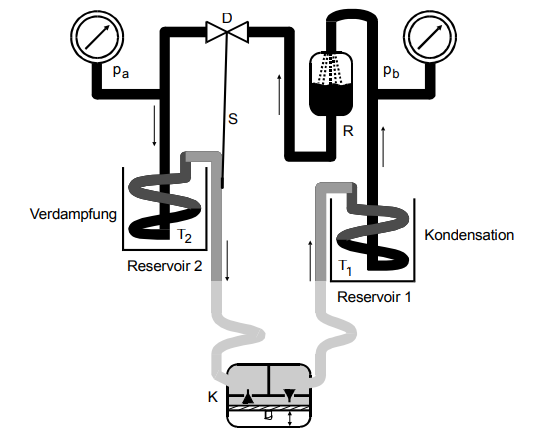
\includegraphics[width=0.4\textwidth]{content/Ausfbau_Skizze_Theorie.png}
	\caption{Skizze zur theoretischen Grundlage der Wärmepumpe.}
	\label{fig:Aufbau_Theorie}
\end{figure}


In der Wärmepumpe wird ein reales Gas als Wärmetransportmedium verwendet. Dieses nimmt beim Verdampfen Energie auf und gibt diese beim Kondensieren wieder ab. Zur Realisierung der 
Wärmepumpe werden meist Gase mit hoher Verdampfungswärme genutzt. In \autoref{fig:Aufbau_Theorie} ist der grundlegende Aufbau einer Wärmepumpe skizziert. Der Kompressor K sorgt für eine Zirkulation 
des Gases durch die Reservoire. Durch das Drosselventil D wird dort ein lokaler Druckunterschied aufgebaut. Dieser Druckunterschied ist so gewählt, das bei beiden Drücken das Gas
einen unterschiedlichen Aggregatzustand annimmt. Beim Verdampfen nach Durchlaufen von D nimmt das Gas die Verdampfungswärme $L$ pro Gramm auf, wodurch also das Reservoir an Energie 
beziehungsweise Wärme verliert. Diese Energie wird dann durch Kondensation im anderen Reservoir abgegeben. Dies geschieht, da der Kompressor K das Gas komprimiert also den Druck erhöht.
Eine Wärmepumpe kann noch durch viele Apperatschaften erweitert und verbessert werden, allerdings wird hier nicht weiter darauf eingegangen. 

\subsection{Kenngrößen einer realen Wärmepumpe}
\label{subsec:Kenngrößen}

Für eine Wärmepumpe nach \autoref{fig:Aufbau_Skizze} gibt es drei relevante Kenngrößen. Eine davon ist die bereits im \autoref{subsec:Prinzip} genannte Güte. Dazu kommen im
Folgenden der Massendurchsatz des Transportmediums $\frac{\text{d}m}{\text{d}t}$ und der Wirkungsgrad $\eta_{\text{K}}$ des Kompressors K. 


In \autoref{subsec:Prinzip} wurde bisher lediglich eine Formel für die theoretische Güte genannt. Die reale Güte $\nu_{\text{real}}$ kann durch 
\begin{equation}
    \label{eqn:Güte_Messung}
    \nu_{\text{real}} = \frac{\left(m_1 c_w + m_k c_k\right)}{N_{\text{mechanisch}}}\frac{\Delta T_1}{\Delta t}
\end{equation}
bestimmt werden. $\frac{\Delta T_1}{\Delta t}$ kann zu einem geeigneten Zeitintervall aus einer Messreihe, welche mit einer Wärmepumpe nach \autoref{fig:Aufbau_Skizze} aufgenommen wird,
errechnet werden. $N_{\text{mechanisch}}$ ist die mittlere Leistung im gewählten Intervall $\Delta t$. $m_1c_w$ beschreibt die Wärmekapazität des Mediums im Reservoir 1 in \autoref{fig:Aufbau_Skizze}. 
$m_kc_k$ beschreibt die Wärmekapazität der Rohrleitungen im Reservoir, welche ebenfalls in \autoref{fig:Aufbau_Skizze} zu sehen sind.


Der Massendurchsatz kann aus der selben Messreihe mit $T_2$ bestimmt werden. 
\begin{equation}
    \label{eqn:Massendurchsatz}
    \frac{\text{d}m}{\text{d}t} = \frac{\left(m_2 c_w + m_k c_k\right)}{L}\frac{\Delta T_2}{\Delta t}
\end{equation}
Die Formel ähnelt \autoref{eqn:Güte_Messung}. Lediglich beschreibt hier der Index 2 das Reservoir 2 und an Stelle von $N_{\text{mechanisch}}$ findet sich ein $L$ 
im Nenner des Bruchs, welches man mit der Kondensationswärme identifiziert.
Diese kann ebenfalls aus der Messreihe per Ausgleichsrechnung bestimmt werden.


Die mechanische Kompressorleistung $N_{\text{mechanisch}}$ erhält man durch
\begin{equation}
    \label{eqn:Leistung}
    N_{\text{mechanisch}} = \frac{1}{\kappa - 1}\left(p_b \sqrt[\kappa]{\frac{p_a}{p_b}} - p_a \right) \frac{1}{\rho} \frac{\text{d}m}{\text{d}t}
\end{equation}
$p_a, p_b$ sind dir Drücke aus \autoref{fig:Aufbau_Skizze}. $\kappa$ ist das Verhältnis der Molwärmen $C_p$ und $C_v$ und $\rho$ beschreibt die Dichte des Transportmediums im gasförmigen
Zustand. Aus der mechanischen Kompressorleistung lässt sich dann der Wirkungsgrad $\eta_K$ bestimmen.